% source https://docs.google.com/presentation/d/1j9GgVLT7fVKHwGSrdbd9HCPcR_T5TcIIF5dhADAEKsk
\begin{figure}

\begin{minipage}[c]{0.2\linewidth}
~
\end{minipage}
~
\begin{minipage}[b]{0.078\linewidth}
    ~
    % 
\includegraphics[width=0.8\linewidth]{{img/fit-key.pdf}}
\end{minipage}%
\begin{minipage}[b]{0.624\linewidth}
        
\includegraphics[width=\linewidth]{{img/fit-key.pdf}}
\end{minipage}

\vspace{1em}

\begin{subfigure}{\linewidth}
\begin{minipage}{0.2\linewidth}
\caption{\footnotesize no biotic background}
\label{fig:fit-nobbg}
\end{minipage}
~
\begin{minipage}{0.78\linewidth}
    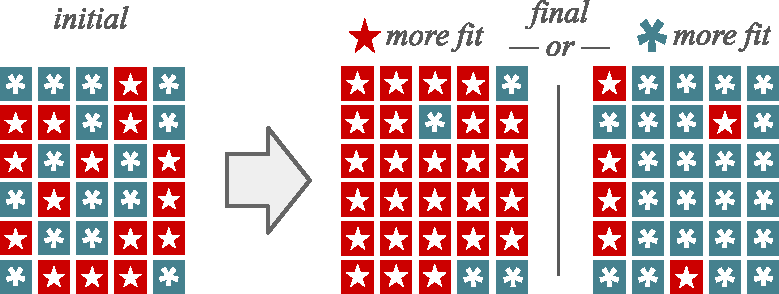
\includegraphics[width=\linewidth]{{img/fit-nobbg.pdf}}
\end{minipage}
\end{subfigure}

\vspace{1em}

\begin{subfigure}{\linewidth}
\begin{minipage}{0.2\linewidth}
\caption{\footnotesize with biotic background}
\label{fig:fit-bbg}
\end{minipage}
~
\begin{minipage}{0.78\linewidth}
    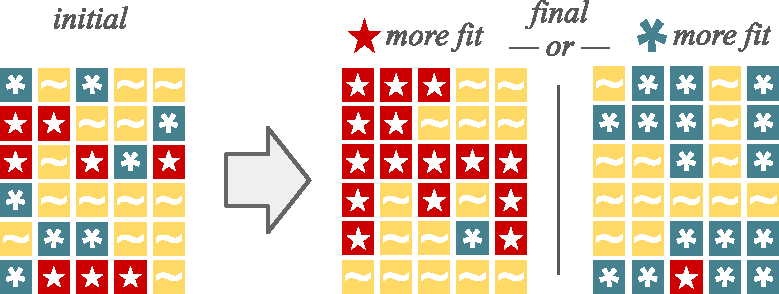
\includegraphics[width=\linewidth]{{img/fit-bbg.pdf}}
\end{minipage}
\end{subfigure}

\caption{%
\textbf{Adaptation assay design.}
\footnotesize
Due to the implicit nature of fitness in our study system, adaptation was primarily assessed on a relative basis, using competition experiments, rather than on an absolute basis.
Panel \ref{fig:fit-nobg} overviews competition experiments design.
For these experiments, population cells are seeded with genomes from two strains, in equal proportion,
After a fixed simulation duration, strain abundances are assessed.
In stint-to-stint adaptation assays, outcome significance was tested according to ``winning'' (higher abundance) strain consistency across replicates.
For genotype/phenotype complexity screens, which required assessment of numerous knockout variants, significance was instead assessed by comparing the end-state abundance ratio against a sampled distribution of outcomes from control WT vs. WT competition replicates.
In some cases, to assess context-sensitivity of fitness, competitions were performed under ``biotic background'' conditions (panel \ref{fig:fit-bg}).
For these competition trials, half the initial population was seeded with a background strain.
}
\label{fig:fit}

\end{figure}
